\capitulo{3}{Conceptos teóricos}

En este apartado voy a comentar los distintos conceptos teóricos del proyecto, que van desde la parálisis cerebral hasta conceptos como \textit{Random Forest}.

\section{Parálisis Cerebral}
Como ya he comentado, la parálisis cerebral es un discapacidad en el sistema motor y en la postura de la persona. Además, esta discapacidad suele ir acompañada de otras discapacidades en el sistema nervioso que producen limitaciones en los sentidos y en la capacidad cognitiva de la persona~\cite{rosenbaum2007report,aspacecyl}.

El origen de esta discapacidad se debe a varios factores, mayoritariamente relacionados con el desarrollo del feto. Además, el grado de afección de la parálisis cerebral es distinto en cada caso, teniendo desde personas levemente afectadas que solo sufren de una discapacidad motora, hasta personas gravemente afectadas con grandes discapacidades motoras, cognitiva, sensoriales...

Existen diversas asociaciones que ayudan a las personas que tienen parálisis cerebral y a las familias, amigos o cualquier persona que acompañe a la persona afectada. Por suerte, en España existen multitud de estas asociaciones, siendo Confederación ASPACE~\cite{aspace} la confederación a nivel nacional. En Castilla y León la asociación es ASPACE Castilla y León, y en Burgos tenemos a APACE Burgos~\ref{fig:apace}~\cite{apace}.
\begin{figure}
	\centering
	
\includegraphics[width=\textwidth]{apace}
	\caption{Logotipo de APACE Burgos a la izquierda y ASPACE CyL a la derecha.}
	\label{fig:apace}
\end{figure}
\section{Señal de audio}
El asistente desarrollado toma como entrada un audio y un conjunto de opciones adicionales que hemos obtenido en colaboración con APACE.
\subsection{Sonido}
Una señal sonora es una  perturbación mecánica (vibraciones) en la presión del aire \cite{pierce1995senales}. Ésta se convierte a una señal eléctrica, en concreto a una señal analógica, que es una señal generada por un fenómeno electromagnético que se puede representar a través de una función continua cuyos parámetros son la amplitud y el periodo \cite{analogica}, mediante un proceso electromagnético. Posteriormente es digitalizada a través de un proceso de muestreo, determinado por la frecuencia de muestreo o \textit{sampling rate}, y de un proceso de cuantificación, que junto con la frecuencia de muestreo determina el \textit{bitrate} de la señal digital. A esta señal almacenada se le llama señal de audio, y esta puede ser obviamente almacenada, reproducida y modificada.
\subsection{Espectrograma}
Es una representación gráfica de las señales de audio, es decir, una representación de las frecuencias de la señal sonora almacenada en la señal analógica que compone la señal de audio~\cite{wiki:espec}. En esta representación la distribución de energía se muestra en tres ejes, siendo el eje de las \textit{x} el eje temporal, el eje de las \textit{y} el de las frecuencias y el color (como eje z) muestra el dominio o la distribución de la señal de audio con respecto a los otros dos ejes, el tiempo y las frecuencias~\cite{granesp}.

Como ya comenté, las señales de audio se caracterizan por su periodo y amplitud, como se puede ver en la representación de la onda en la figura~\ref{fig:onda}. En cambio, el espectrograma de éste se muestra en la figura~\ref{fig:espec} en una escala lineal, y en una escala logarítmica en la figura~\ref{fig:especlog}.
\begin{figure}
	\centering
	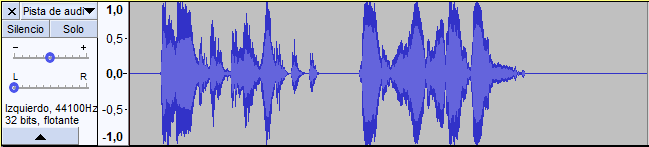
\includegraphics[width=\textwidth]{onda}
	\caption{Representación de la onda. En el eje \textit{x} se representa el tiempo y en el eje \textit{y} la amplitud.}
	\label{fig:onda}
\end{figure}
\begin{figure}
	\centering
	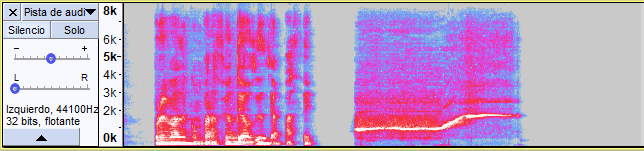
\includegraphics[width=\textwidth]{especlineal}
	\caption{Espectrograma en escala lineal. En el eje \textit{x} se representa el tiempo y en el eje \textit{y} la componente espectral (frecuencia) en escala lineal.}
	\label{fig:espec}
\end{figure}
\begin{figure}
	\centering
	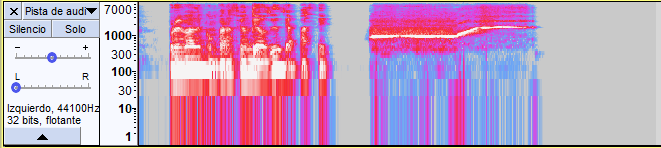
\includegraphics[width=\textwidth]{especlog}
	\caption{Espectrograma en escala logarítmica. En el eje \textit{x} se representa el tiempo y en el eje \textit{y} la componente espectral (frecuencia) en escala logarítmica.}
	\label{fig:especlog}
\end{figure}
\subsection{Frecuencias en escala de Mel, MFCC} \label{mel}
Es una escala que surgió con el objetivo de obtener una escala orientada al sistema auditivo del ser humano, lo que se llama una escala psicoacústica. Su finalidad es poder extraer características de la señal de audio para obtener información. Podemos ver el ejemplo del mismo audio en la figura~\ref{fig:mel}

Esta es la fórmula de las frecuencias en escala de Mel y las frecuencias en escala lineal (f)\cite{wiki:mel,villa2012automatic}: \[ Mel(f) = 2595 * \log_{10}(1+\frac{f}{700})\]

MFCC (\textit{Coeficientes Cepstrales en las Frecuencias de Mel}) son los coeficientes necesarios para esta representación del sonido relacionado con el sistema auditivo humano. El proceso de obtención de este coeficiente sigue los siguientes pasos~\cite{wiki:mel,yeo2011animal}:
\begin{itemize}
	\item División del audio en fragmentos (\textit{frames}).
	\item Minimizar las discontinuidades de la señal en el comienzo y final de cada fragmento.
	\item Aplicar la Transformada Discreta de \textit{Fourier} para conseguir la potencia espectral.
	\item Aplicar los filtros correspondientes a la escala de \textit{Mel}.
	\item De cada frecuencia de \textit{Mel} de las energías obtenemos el logaritmo.
	\item Aplicamos la transformada de coseno discreta a los logaritmos.
\end{itemize}
\begin{figure}
	\centering
	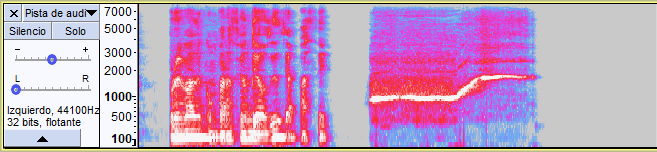
\includegraphics[width=\textwidth]{mel}
	\caption{Espectrograma en escala de Mel. En el eje \textit{x} se representa el tiempo, en el eje \textit{y} las frecuencias relativas a la capacidad auditiva humana.}
	\label{fig:mel}
\end{figure}

\subsection{Zero Crossing Rate} \label{zcr}
Es el ratio que mide el número de veces en las cuales la señal cambia de signo.
\subsection{Bitrate}
Es la unidad de datos que se recogen por unidad de tiempo. Los datos recogidos se miden en bits, mientras que el tiempo se mide en segundos.
Cuando trabajamos con sistemas de recogida de datos, en nuestro caso grabaciones de audios, el \textit{bitrate} de esta recogida es un valor muy importante, ya que determina la cantidad de datos que vamos a obtener. Esta medida puede ser muy interesante a la par de necesaria ya que, junto con el formato y el códec, va a determinar cuánto ocupan los archivos que obtenemos además de la calidad de estos.
\subsection{Sampling Rate}
El Sampling Rate o frecuencia de muestreo es la tasa que marca la cantidad de muestras que se hacen por unidad de tiempo. Partiendo de nuestra función continua, que es la señal analógica, que recoge la señal sonora, es decir, la señal de audio, pasamos a valores discretos. La unidad con la que se mide es, como en todas las frecuencias, $s^{-1}$ o \textit{Hz}~\cite{wiki:sampling}.

\subsection{Formato digital}
Dentro de una señal de audio, y en general para cualquier tipo de dato que se almacena de forma digital, el formato es el estándar, con el cual el dato se codifica, se decodifica y se lee.

Dentro de los formatos que existen en las señales de audios o formatos contenedores de audios podemos diferenciarlos entre los que tienen pérdida de información o \textit{Lossy} y los que no la tienen o \textit{Loseless}. Los formatos que tienen pérdida suelen ser formatos más ligeros, en los cuales los ficheros ocupan menos y son más fáciles de procesar. En cambio, como su nombre indica, tienen pérdidas de información~\cite{wiki:formatoaudio}. 
\subsection{Encoder}
El encoder o códec son los métodos por los cuales podemos codificar y decodificar los datos de audios almacenados en el formato seleccionado. Para cada códec disponemos de una serie de formatos en los cuales se puede codificar y decodificar, por lo que en si, la combinación códec-formato es la que puede ser \textit{Lossy} o \textit{Loseless}~\cite{wiki:codec}.

La mayoría de códecs son  \textit{Lossy}, es decir, pierden información en la codificación que luego no se puede recuperar en la decodificación, alguno de los códecs de audios más usados son los que se pueden observar en la tabla~\ref{tabla:codecaudio}.
\tablaSmall{Códecs de audio}{l c c}{codecaudio}
{ \multicolumn{1}{l}{\textbf{Códecs}} & \textbf{\textit{Lossy}} & \textbf{\textit{Loseless}} \\}{ 
	AAC-LC & X &\\
	AAC-ELD & X &\\
	HE-AAC & X &\\
	AMR-NB & X &\\
	AMR-WB & X &\\
	PCM(Pulse Code Modulations) & & X\\
	FLAC & & X\\
} 
\subsection{Base64}
Método que nos permite codificar cualquier tipo de dato y/o archivo en texto ASCII y decodificarlo. Este tipo de codificación no es la más eficiente que existe, pero si que nos puede servir si queremos mandar nuestros ficheros en modo texto, como pasa en este proyecto, donde tenemos que enviar el audio grabado al servidor a través de un método post donde las variables se pasan en la URL.
\subsection{Extracción de características}
Proceso por el cual podemos obtener información a partir de datos. Se suele llevar a cabo en el preprocesado de información de entrada de los métodos de clasificación de minería de datos, ya que datos como pueden ser imágenes, o en nuestro caso audios, no las podemos pasar tal cual al clasificador porque no sería capaz de interpretar la entrada, y si por un casual pudiese, ésta tendría una gran dimensionalidad.

En nuestro caso, del audio se obtienen los 500 \textit{frames} que se van a estudiar y de estos 500 se obtienen los 12 primeros coeficientes de \textit{MFCC}~\ref{mel} y su \textit{Zero Crossing Rate}~\ref{zcr}. Pero no podemos pasarle a nuestro clasificador una matriz de 500x13, por lo que convertimos esta matriz en una única fila con 26 columnas, que son las 12 medias de los coeficientes de \textit{MFCC}, las 12 desviaciones estándar de los coeficientes de \textit{MFCC}, la media del \textit{Zero Crossing Rate} y su desviación estándar.

\section{Minería de Datos, Bagging y Random Forest}
La minería de datos tiene diversas definiciones válidas, pero todas ellas coinciden en que es un proceso en el cual, a partir de grandes cantidades de datos a los que se aplican técnicas de inteligencia artificial o de análisis de datos, podemos obtener patrones, relaciones o en definitiva información, con la que podemos clasificar o dividir en grupos nuevos datos.

La minería de datos entra dentro del apartado de aprendizaje automática, entendiendo como aprendizaje cuando en un sistema cambiamos el comportamiento de alguna parte o del conjunto y obtenemos una mejora en el rendimiento.

La extracción de información de la minería de datos se basa en la hipótesis de \textit{Aprendizaje Inductivo}, que es "\textit{Cualquier modelo que aproxime bien una función objetivo sobre un conjunto de ejemplos de entrenamiento suficientemente grande también aproximará bien la función objetivo en ejemplos no observados}", es decir, los patrones encontrados en los datos de entrenamiento de nuestros modelos de minería de datos, con un número suficientemente grande de datos, servirá para nuevos datos del mismo tipo~\cite{mdintro}.

Los métodos de minería de datos tienen distintas finalidades entre las que se destaca:
\begin{itemize}
	\item Predicción:
	\begin{itemize}
		\item Clasificación de datos categóricos.
		\item Regresión de datos numéricos.
	\end{itemize}
	\item Análisis de asociaciones entre los atributos que definen los datos.
	\item Clustering o agrupación de los datos en distintos grupos.
	\item Detección de anomalías.
	\item Sistema de recomendaciones.
\end{itemize}

Además, dentro de la minería de datos existen diferentes métodos para llegar a las finalidades anteriormente comentadas. Estos tipos de algoritmos van desde métodos basados en árboles hasta métodos más estadísticos como los modelos de clasificación bayesiana que usan la suposición de \textit{naïve}, en la cual se supone que los atributos de los datos no tienen ninguna relación~\cite{mdrf}.

Dentro de los algoritmos de minería de datos hay una serie de técnicas que nos permiten combinar varios modelos clasificadores para obtener un único modelo, \textit{ensembles}, que aunque son más complejos de representar pueden obtener mejores resultados. La combinación de modelos puede o no ser del mismo tipo de clasificador, es decir, hay técnicas que nos permiten usar por ejemplo métodos bayesianos con árboles y otros que solo nos permiten un mismo tipo de clasificador. Una de las técnicas más usadas de combinación de métodos es \textit{Bagging}. Ésta consiste en la combinación mediante media en problemas de regresión y mediante votación en problemas de clasificación, de los resultados obtenidos por el mismo método. A partir de varios grupos de datos o muestras del mismo problema, el algoritmo obtiene para cada muestra un modelo entrenado con los datos de esa muestra. El método final lo que hace es combinar los resultados, por media o votación, de los distintos modelos de las diferentes muestras.

Uno de los métodos de \textit{Bagging} más usados, ya que es un método sencillo que nos puede dar una primera visión del problema ante el que estamos, es \textit{Random Forest}, en el cual combinamos las predicciones de distintos árboles de decisión. Usa como estimador del error el \textit{out of bag}, que consiste en intentar predecir con cada modelo los datos de las muestras con los que no se ha entrenado ese modelo~\cite{mdrf}.